%%%%%%%%%%%%%%%%%%%%%%%%%%%%%%%%%%%%%%%%%%%%%%%%%%%%%%%%%%%%%%%%
% %
% Seth Cram %
% ECE351 Section 53 %
% Lab 12 %
% Due 04/26/2022 %
% Any other necessary information needed to navigate the file %
%
%
% %
%%%%%%%%%%%%%%%%%%%%%%%%%%%%%%%%%%%%%%%%%%%%%%%%%%%%%%%%%%%%%%%%
%%%%%%%%%%%%%%%%%%%%%%%%%%%%%%%%%%%%%%%%%%%
%%% DOCUMENT PREAMBLE %%%
\documentclass[12pt]{report}
\usepackage[english]{babel}
%\usepackage{natbib}
\usepackage{url}
\usepackage[utf8x]{inputenc}
\usepackage{amsmath}
\usepackage{graphicx}
\graphicspath{{images/}}
\usepackage{parskip}
\usepackage{fancyhdr}
\usepackage{vmargin}
\usepackage{listings}
\usepackage{hyperref}
\usepackage{xcolor}
\usepackage{verbatim}
\usepackage{listings}

\definecolor{codegreen}{rgb}{0,0.6,0}
\definecolor{codegray}{rgb}{0.5,0.5,0.5}
\definecolor{codeblue}{rgb}{0,0,0.95}
\definecolor{backcolour}{rgb}{0.95,0.95,0.92}

\begin{comment} %have to use verbatim package for this

\section{Personal Notes}
            


\end{comment}

\lstdefinestyle{mystyle}{
    backgroundcolor=\color{backcolour},   
    commentstyle=\color{codegreen},
    keywordstyle=\color{codeblue},
    numberstyle=\tiny\color{codegray},
    stringstyle=\color{codegreen},
    basicstyle=\ttfamily\footnotesize,
    breakatwhitespace=false,         
    breaklines=true,                 
    captionpos=b,                    
    keepspaces=true,                 
    numbers=left,                    
    numbersep=5pt,                  
    showspaces=false,                
    showstringspaces=false,
    showtabs=false,                  
    tabsize=2
}
 
\lstset{style=mystyle}

\setmarginsrb{3 cm}{2.5 cm}{3 cm}{2.5 cm}{1 cm}{1.5 cm}{1 cm}{1.5 cm}

\title{Lab 12}		%TITLE						
% Title
\author{ Seth Cram}						
% Author
\date{04/26/2022}
% Date

\makeatletter
\let\thetitle\@title
\let\theauthor\@author
\let\thedate\@date
\makeatother

\pagestyle{fancy}
\fancyhf{}
\rhead{\theauthor}
\lhead{\thetitle}
\cfoot{\thepage}
%%%%%%%%%%%%%%%%%%%%%%%%%%%%%%%%%%%%%%%%%%%%
\begin{document}

%%%%%%%%%%%%%%%%%%%%%%%%%%%%%%%%%%%%%%%%%%%%%%%%%%%%%%%%%%%%%%%%%%%%%%%%%%%%%%%%%%%%%%%%%

\begin{titlepage}
	\centering
    \vspace*{0.5 cm}
   % \includegraphics[scale = 0.075]{bsulogo.png}\\[1.0 cm]	% University Logo
\begin{center}    \textsc{\Large   ECE 351 - 53 }\\[2.0 cm]	\end{center}% University Name
	\textsc{\Large  }\\[.5 cm]				% Course Code
	\rule{\linewidth}{0.2 mm} \\[0.4 cm]
	{ \huge \bfseries \thetitle}\\
	\rule{\linewidth}{0.2 mm} \\[1.5 cm]
	
	\begin{minipage}{0.4\textwidth}
		\begin{flushleft} \large
		%	\emph{Submitted To:}\\
		%	Name\\
          % Affiliation\\
           %contact info\\
			\end{flushleft}
			\end{minipage}~
			\begin{minipage}{0.4\textwidth}
            
			\begin{flushright} \large
			\emph{Submitted By :} \\
			Seth Cram  
		\end{flushright}
           
	\end{minipage}\\[2 cm]
	
\end{titlepage}

%%%%%%%%%%%%%%%%%%%%%%%%%%%%%%%%%%%%%%%%%%%%%%%%%%%%%%%%%%%%%%%%%%%%%%%%%%%%%%%%%%%%%%%%%

\tableofcontents
\pagebreak

%%%%%%%%%%%%%%%%%%%%%%%%%%%%%%%%%%%%%%%%%%%%%%%%%%%%%%%%%%%%%%%%%%%%%%%%%%%%%%%%%%%%%%%%%
\renewcommand{\thesection}{\arabic{section}}

\section{Introduction}

The goal of lab 12 is to apply the skills and concepts from Signals and Systems into a practical application using Python in the Spyder IDE and present the information in a professional report.

\section{Equations}
    \begin{equation*}
        H(s) = \frac{\frac{1}{RC}s}{s^2+\frac{1}{RC}s+\frac{1}{LC}} 
    \end{equation*}
    \begin{equation*}
        R = 5\Omega
    \end{equation*}
    \begin{equation*}
        L = 1mH
    \end{equation*}
    \begin{equation*}
        C = 8uF
    \end{equation*}
    
\section{Methodology}

%This section will describe how you went about solving the lab. Make sure you go into detail about any method you used. %Include coding samples here if necessary. This is also where you would include necessary derivations. An example of %inserting code into the report is given. Do not go overboard on inserting code into your report, only use whats %absolutely necessary to illustrate your point.

    \paragraph{} First, I noted the expected 16 or more total plots. Then, I took note of the desired signal frequency of between 1.8kHz ≤ f ≤ 2.0kHz. Next, I inscribed how the switching amplifier should cause noise at higher frequencies. For the next requirement, I needed to attenuate the unwanted low frequency vibrations. 
    
    \paragraph{} With requirements in hand, I used the code provided by the lab handout to read the input signal from a file. I then identified the magnitudes and corresponding frequencies of the position measurement using a fast fourier transform (fft). Reusing the clean fft function created in lab 9 and the provided make stem function, I plotted all the areas that the requirements specified in step 2. 
    
    \paragraph{} Next, I designed an analog filter circuit to remove the noise and only pass the position measurement information. Realizing I needed a bandpass filter, I looked back at lab 10 and decided to alter the component values and shift the bandpass filter for my needs. The circuit's corresponding schematic is seen in the Results section of this report. Component values are listed below the schematic and within the Equations section. 
    
    \paragraph{}Taking the specifications our filter must meet, I crafted multiple graphs targeted at each area of concern of the bode magnitude plot. Lab 10 helped once again in this regard. 
    
    \paragraph{} Finally, I ran my input signal through the transfer function. Taking the fft of the output signal, I created several plots once again targeted toward each problem area. Comparing each problem area's pre and post filter proved that my filter worked perfectly. 
    
\section{Results}

%This section will go over the results of the lab. Use this area to describe %if the lab worked as expected or if the results are unexpected or different %from your hand calculations or intuition. Part of being a good engineer is %gaining intuition about these problems and being able to understand quickly %if something is wrong. Use code, plots, tables, and figures as necessary. %Make sure to cite all other works used and note them in the bibliography. A %sample entry is in this document.
    
    \paragraph{} My expectations for the transfer function were an RLC circuit. I wasn't sure how the variation in the component values would affect the band-pass filter.  
    
    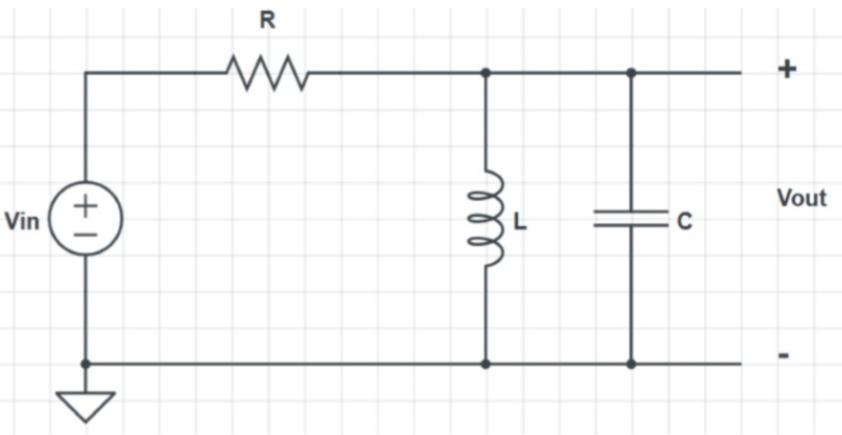
\includegraphics[]{RLC.PNG}
    
    \paragraph{} $R = 5\Omega$, $L = 1mH$, $C = 8uF$
    
    \paragraph{} As seen above, my expectation for the filter being an RLC circuit proved true. Testing different component values, I was able to determine their following effects on the filter:
    
    \begin{enumerate}
        \item Decreasing R resulted in a shallower slope, less overall attenuation, and no shifting.
        \item Decreasing C resulted in a shallower slope and a right shift.
        \item Decreasing L resulted in a steeper slope and right shift.
    \end{enumerate}
    
    \paragraph{} Of course, increasing the component values would do the opposite of what's mentioned above. 
    
    \paragraph{} For the input signal, I plotted it for reference before filtering and completely raw. A large amount of noise is present throughout its breadth that I'll need to filter out. 
    
    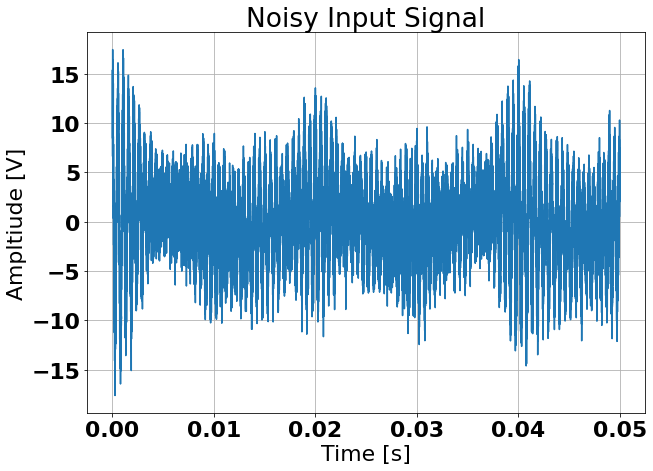
\includegraphics[scale = 0.5]{Figure 2022-04-20 163927 (0).png}
    
    \paragraph{} The output signal is shown next.
    
    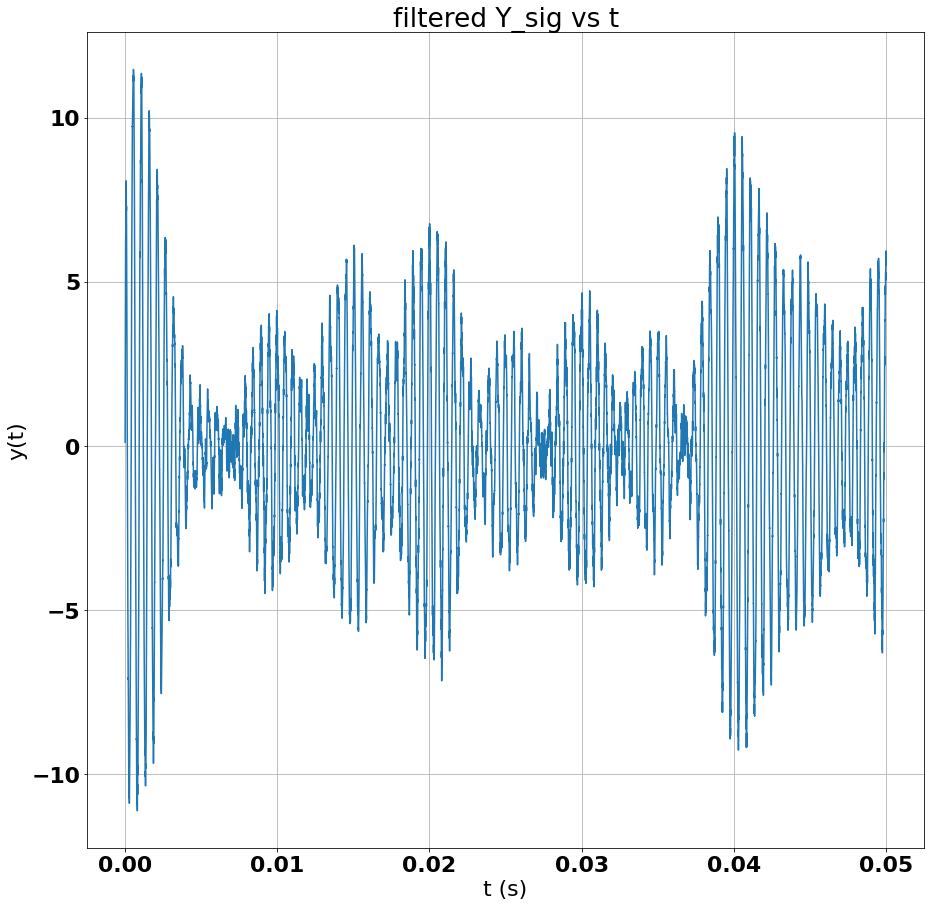
\includegraphics[scale = 0.3]{Figure 2022-04-20 163927 (11).png}
    
    \paragraph{} Even though it doesn't reach the same magnitudes as the input signal, I'm not concerned since the filter should attenuate a great deal of the noise.
    
    \paragraph{} Overall comparison pre and post filter will now be done. I'll first present the bode plot with the magnitude, then the pre-filter signal and post-filter signal. 
    
    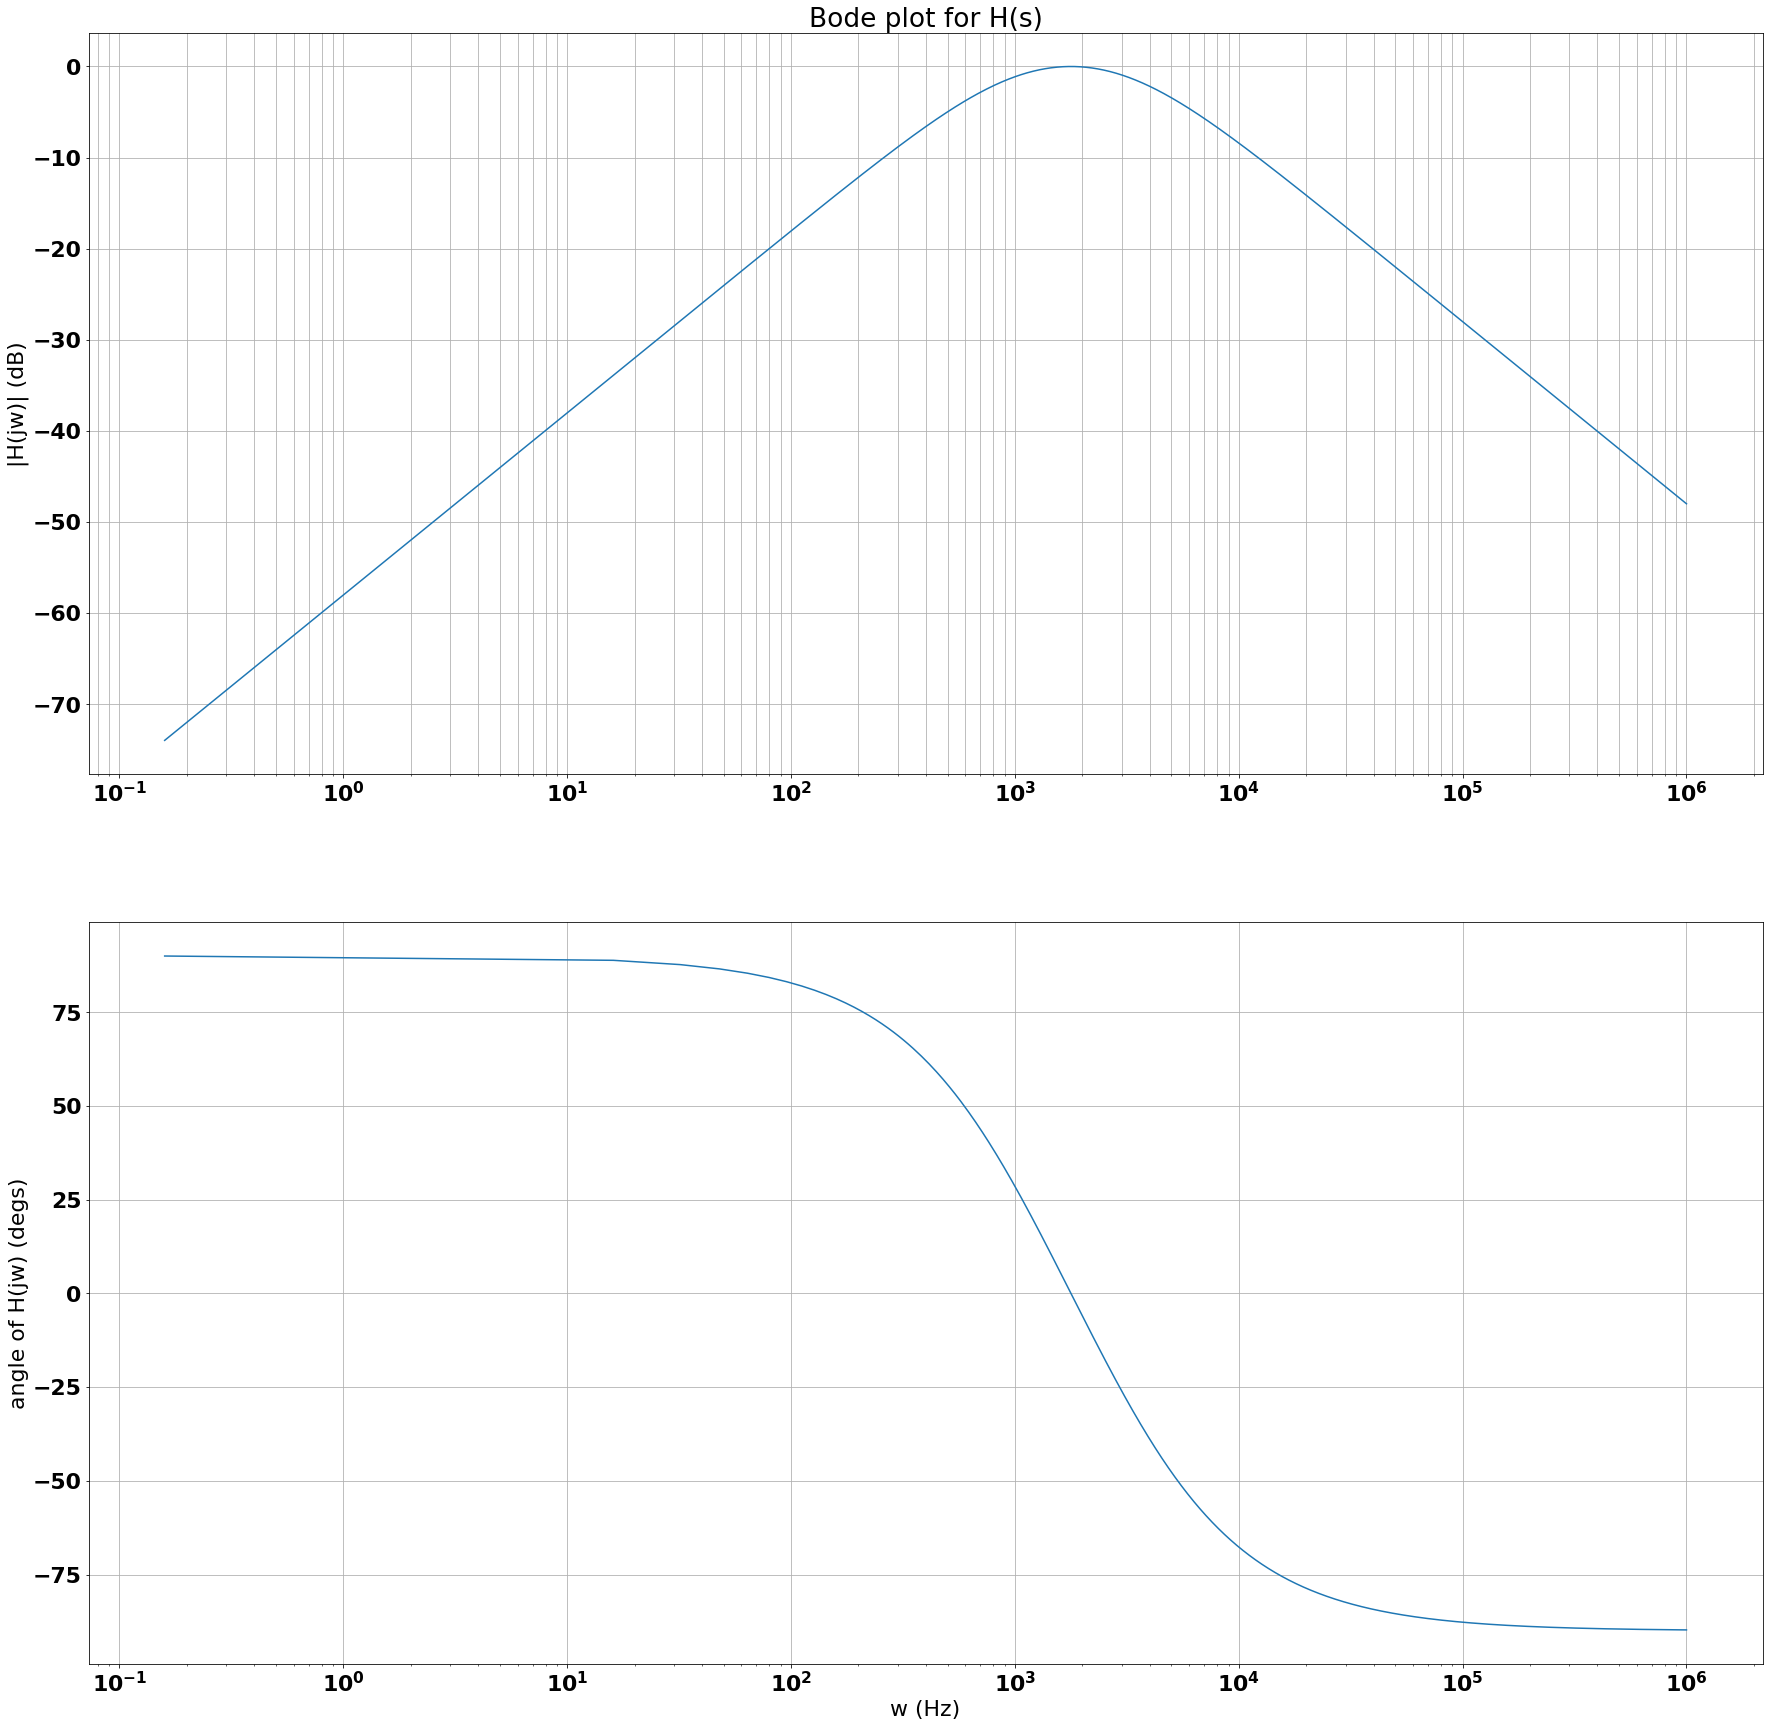
\includegraphics[scale = 0.2]{Figure 2022-04-20 163927 (6).png}
    
    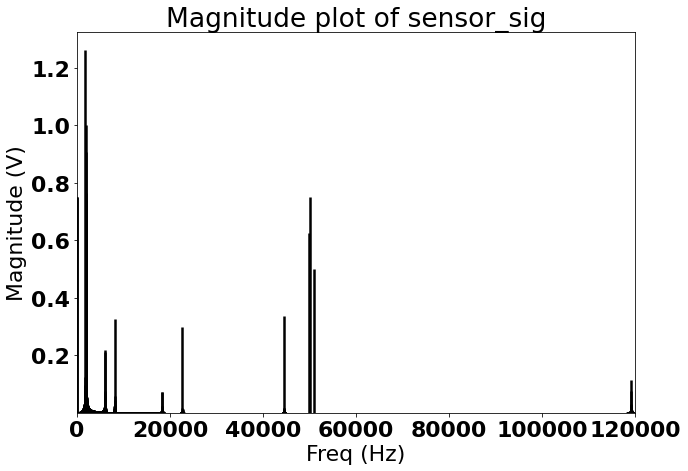
\includegraphics[scale = 0.5]{Figure 2022-04-20 163927 (1).png}
    
    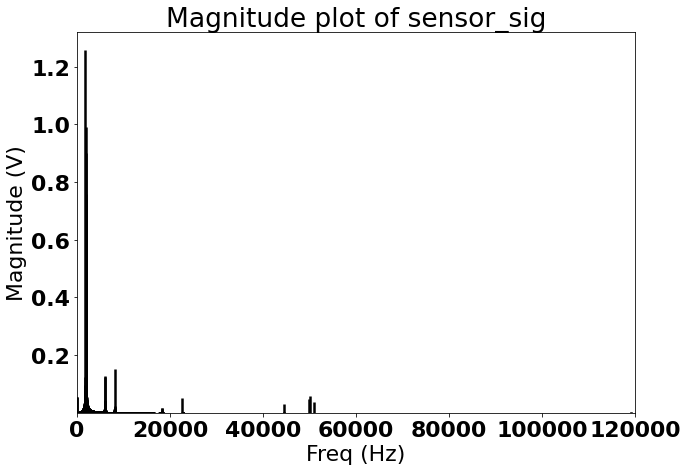
\includegraphics[scale = 0.5]{Figure 2022-04-20 163927 (12).png}
    
    \paragraph{} At a quick glance, the band-pass filter zeroes out around the 2kHz range and relatively steep slope. Just the shape desired. The phase plot is included for completeness but unnecessary for this project's completion. 
    
    \paragraph{} As seen above, the noise at higher frequencies is greatly attenuated after passing the sensor signal through the filter.
    
    \paragraph{} For the first problem area, we're concerned with the position measurement information being attenuated by less than -0.3dB.
    
    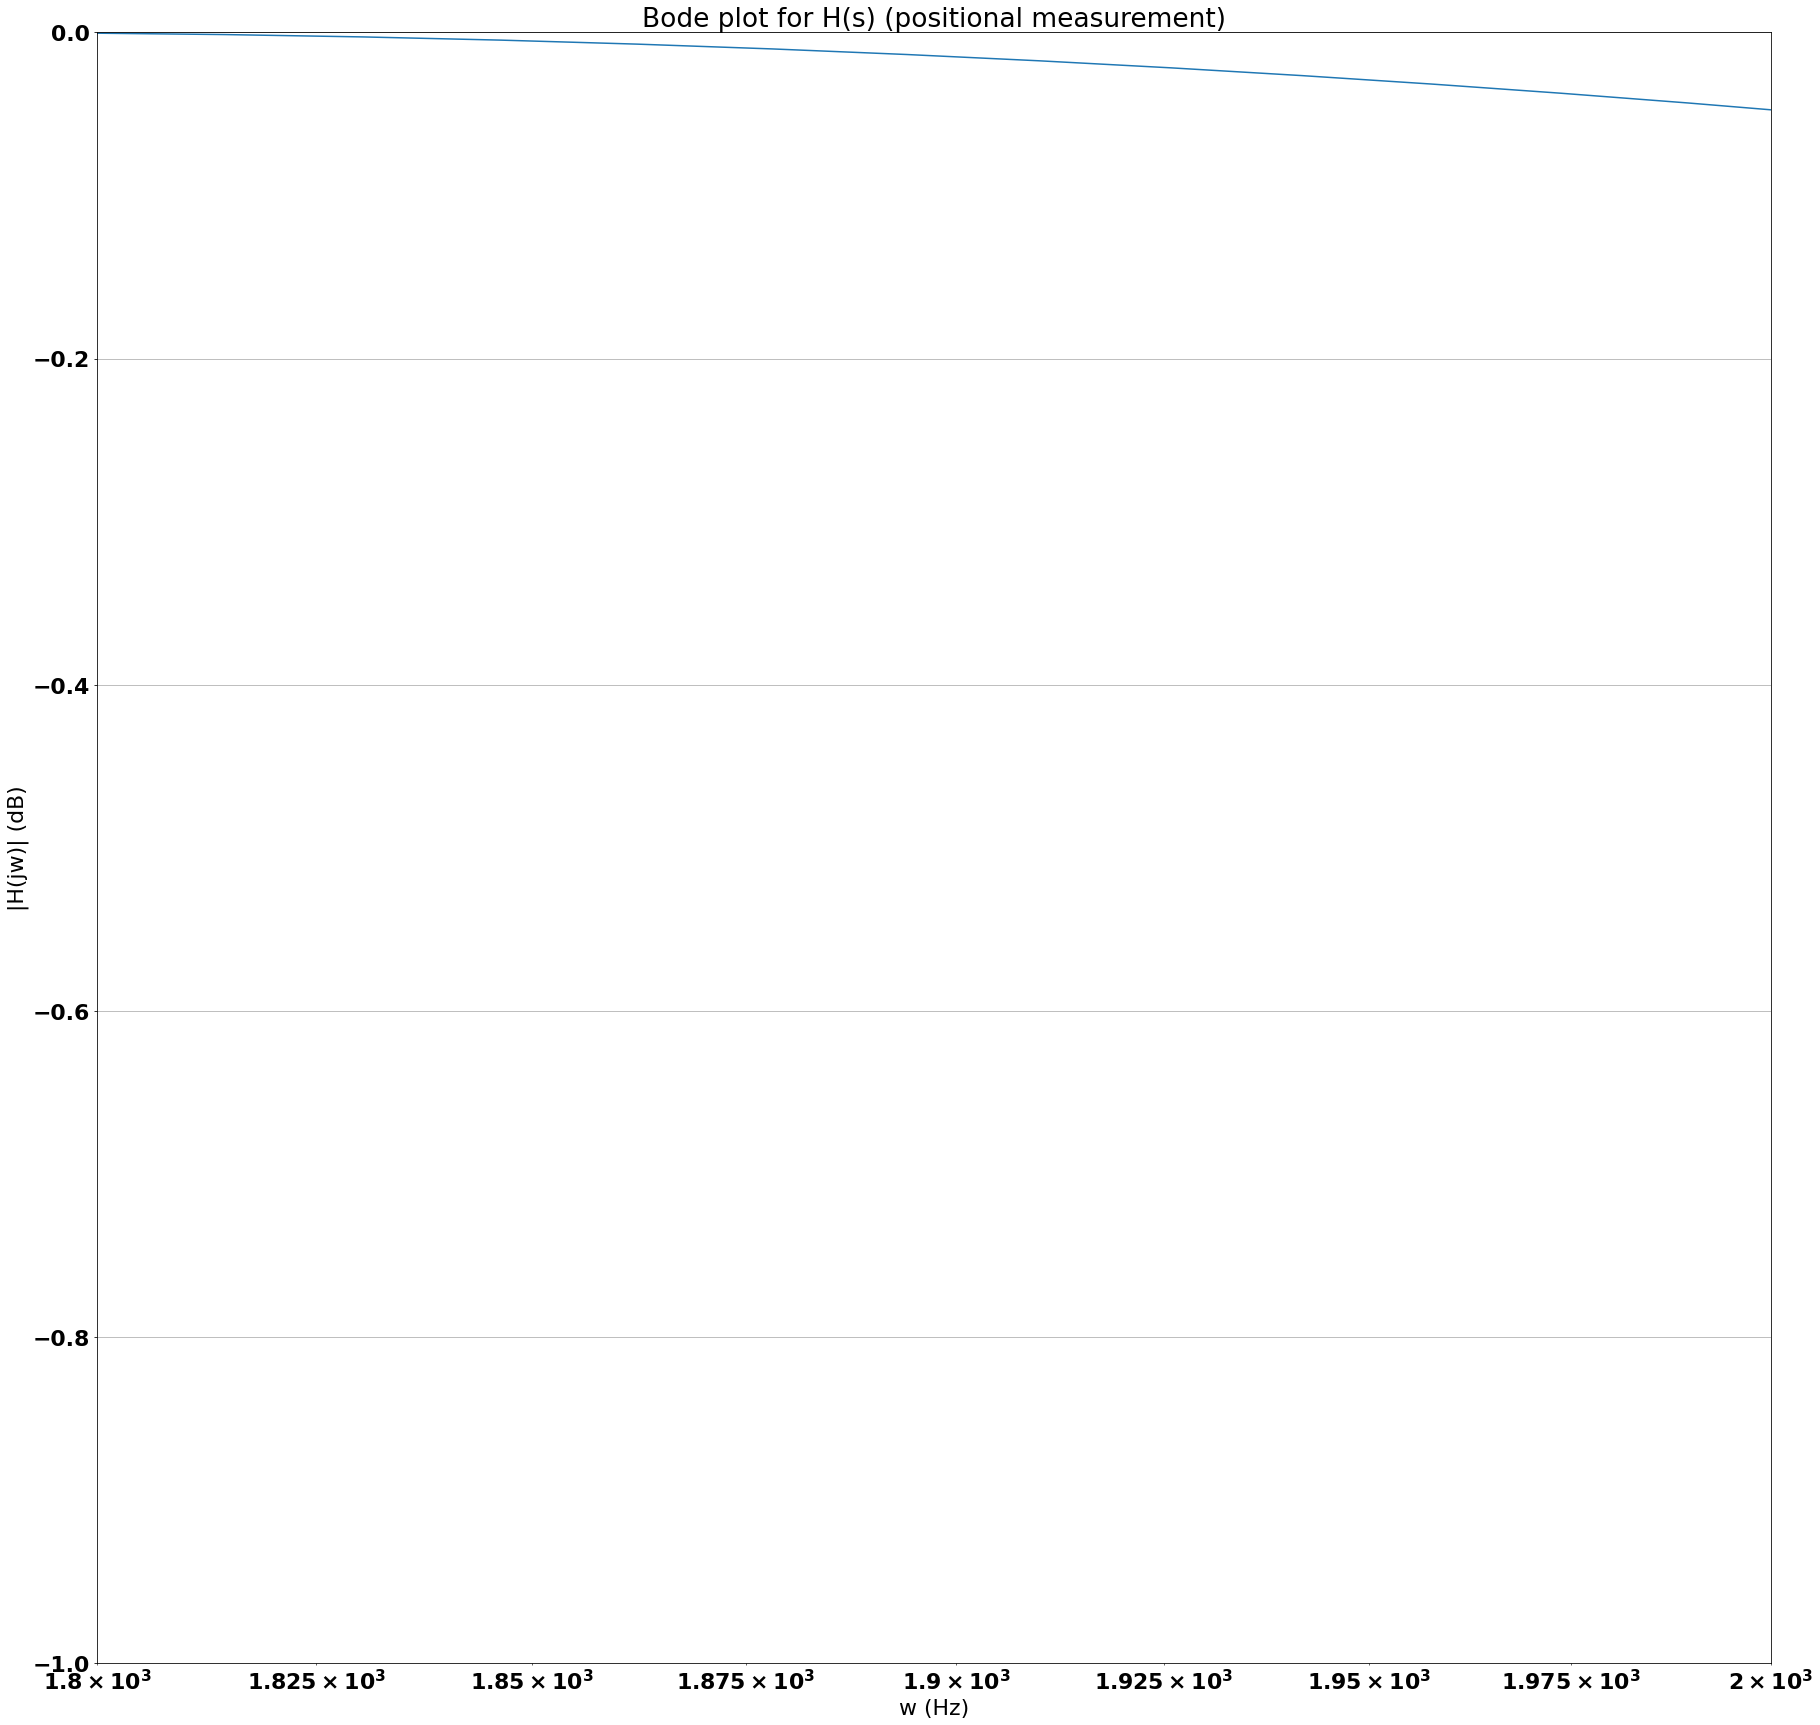
\includegraphics[scale = 0.2]{Figure 2022-04-20 163927 (8).png}
    
    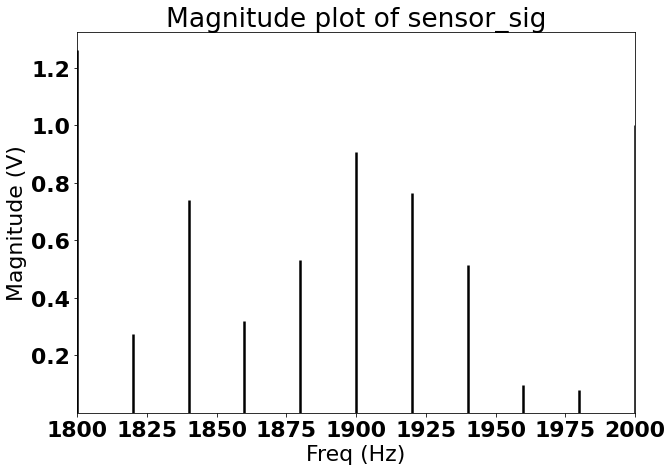
\includegraphics[scale = 0.5]{Figure 2022-04-20 163927 (2).png}

    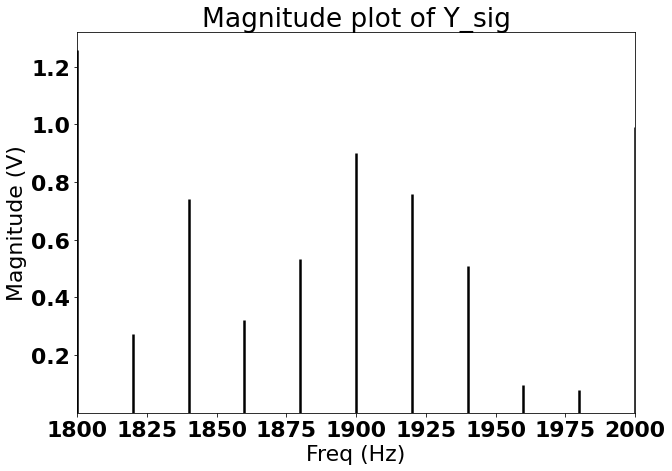
\includegraphics[scale = 0.5]{Figure 2022-04-20 163927 (13).png}
    
    \paragraph{} The bode plot shows how little attenuation the input signal goes through within the 1.8kHz to 2kHz range. It falls within specifications, attenuating less than -0.3dB. As proof, we can see how the output signal and input signal are nearly identical. 
    
    \paragraph{} For the second problem area, we're concerned with the low-frequency vibration noise being attenuated by at least -30dB.
    
    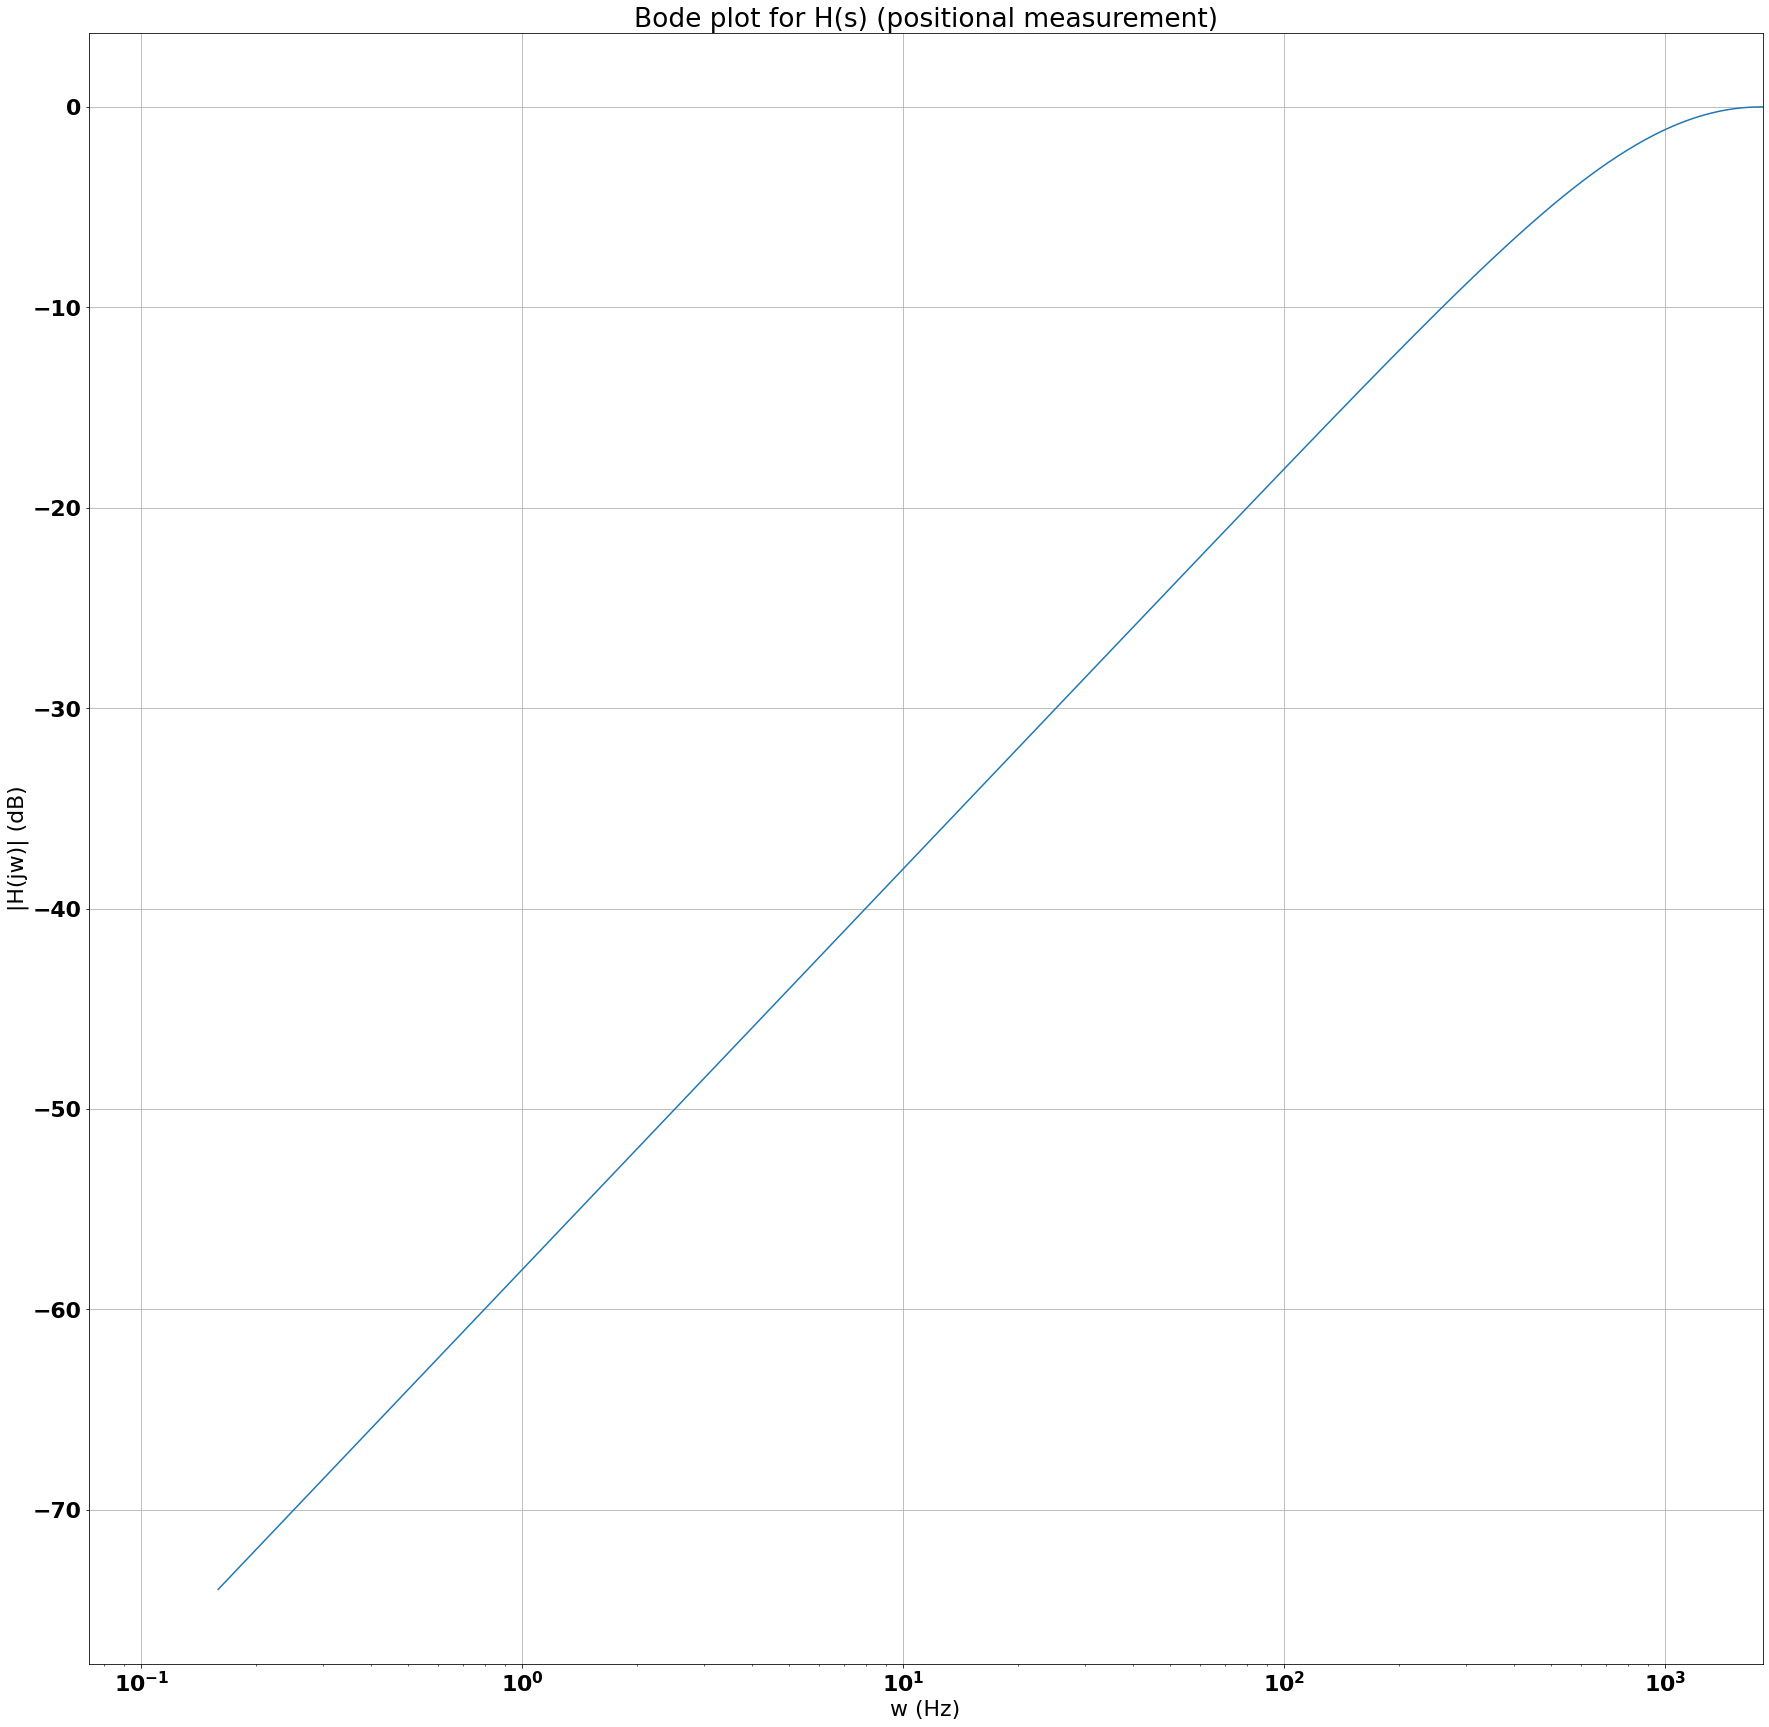
\includegraphics[scale = 0.2]{Figure 2022-04-20 163927 (7).png}
    
    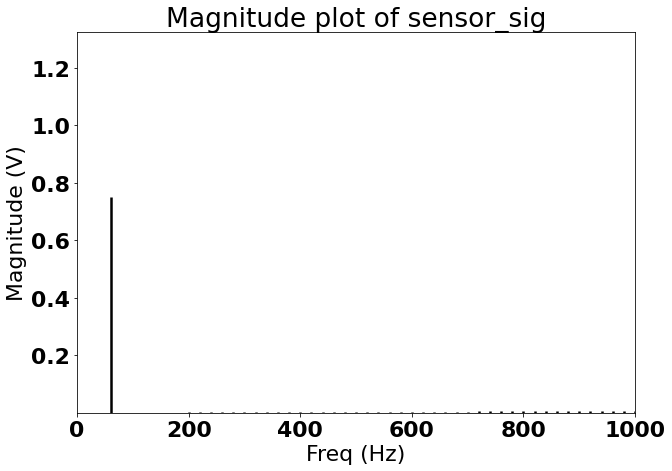
\includegraphics[scale = 0.5]{Figure 2022-04-20 163927 (3).png}

    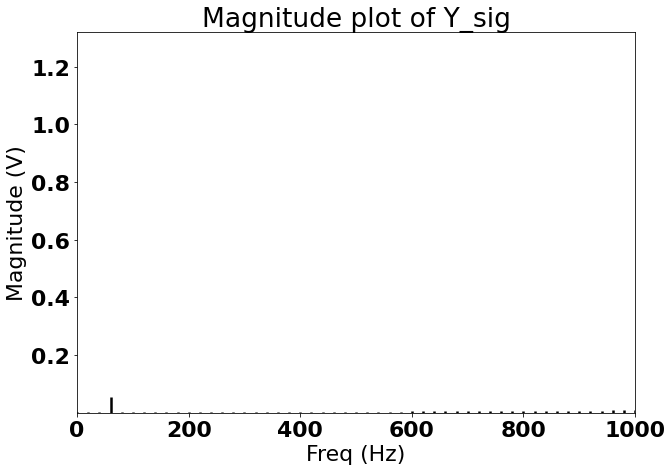
\includegraphics[scale = 0.5]{Figure 2022-04-20 163927 (14).png}
    
    \paragraph{} The bode plot shows how by around 50 Hz, the signal should be attenuated by -30dB. The 50 Hz mark is important because it's the most prominent low frequency noise in our signal. It gets attenuated from a magnitude of 0.7V to 0.05V. 
    
    \paragraph{} For the third problem area, we're concerned with the switching amplifier noise being attenuated by at least -21dB. So, we're concerned with large magnitude spikes after the target frequency range.
    
    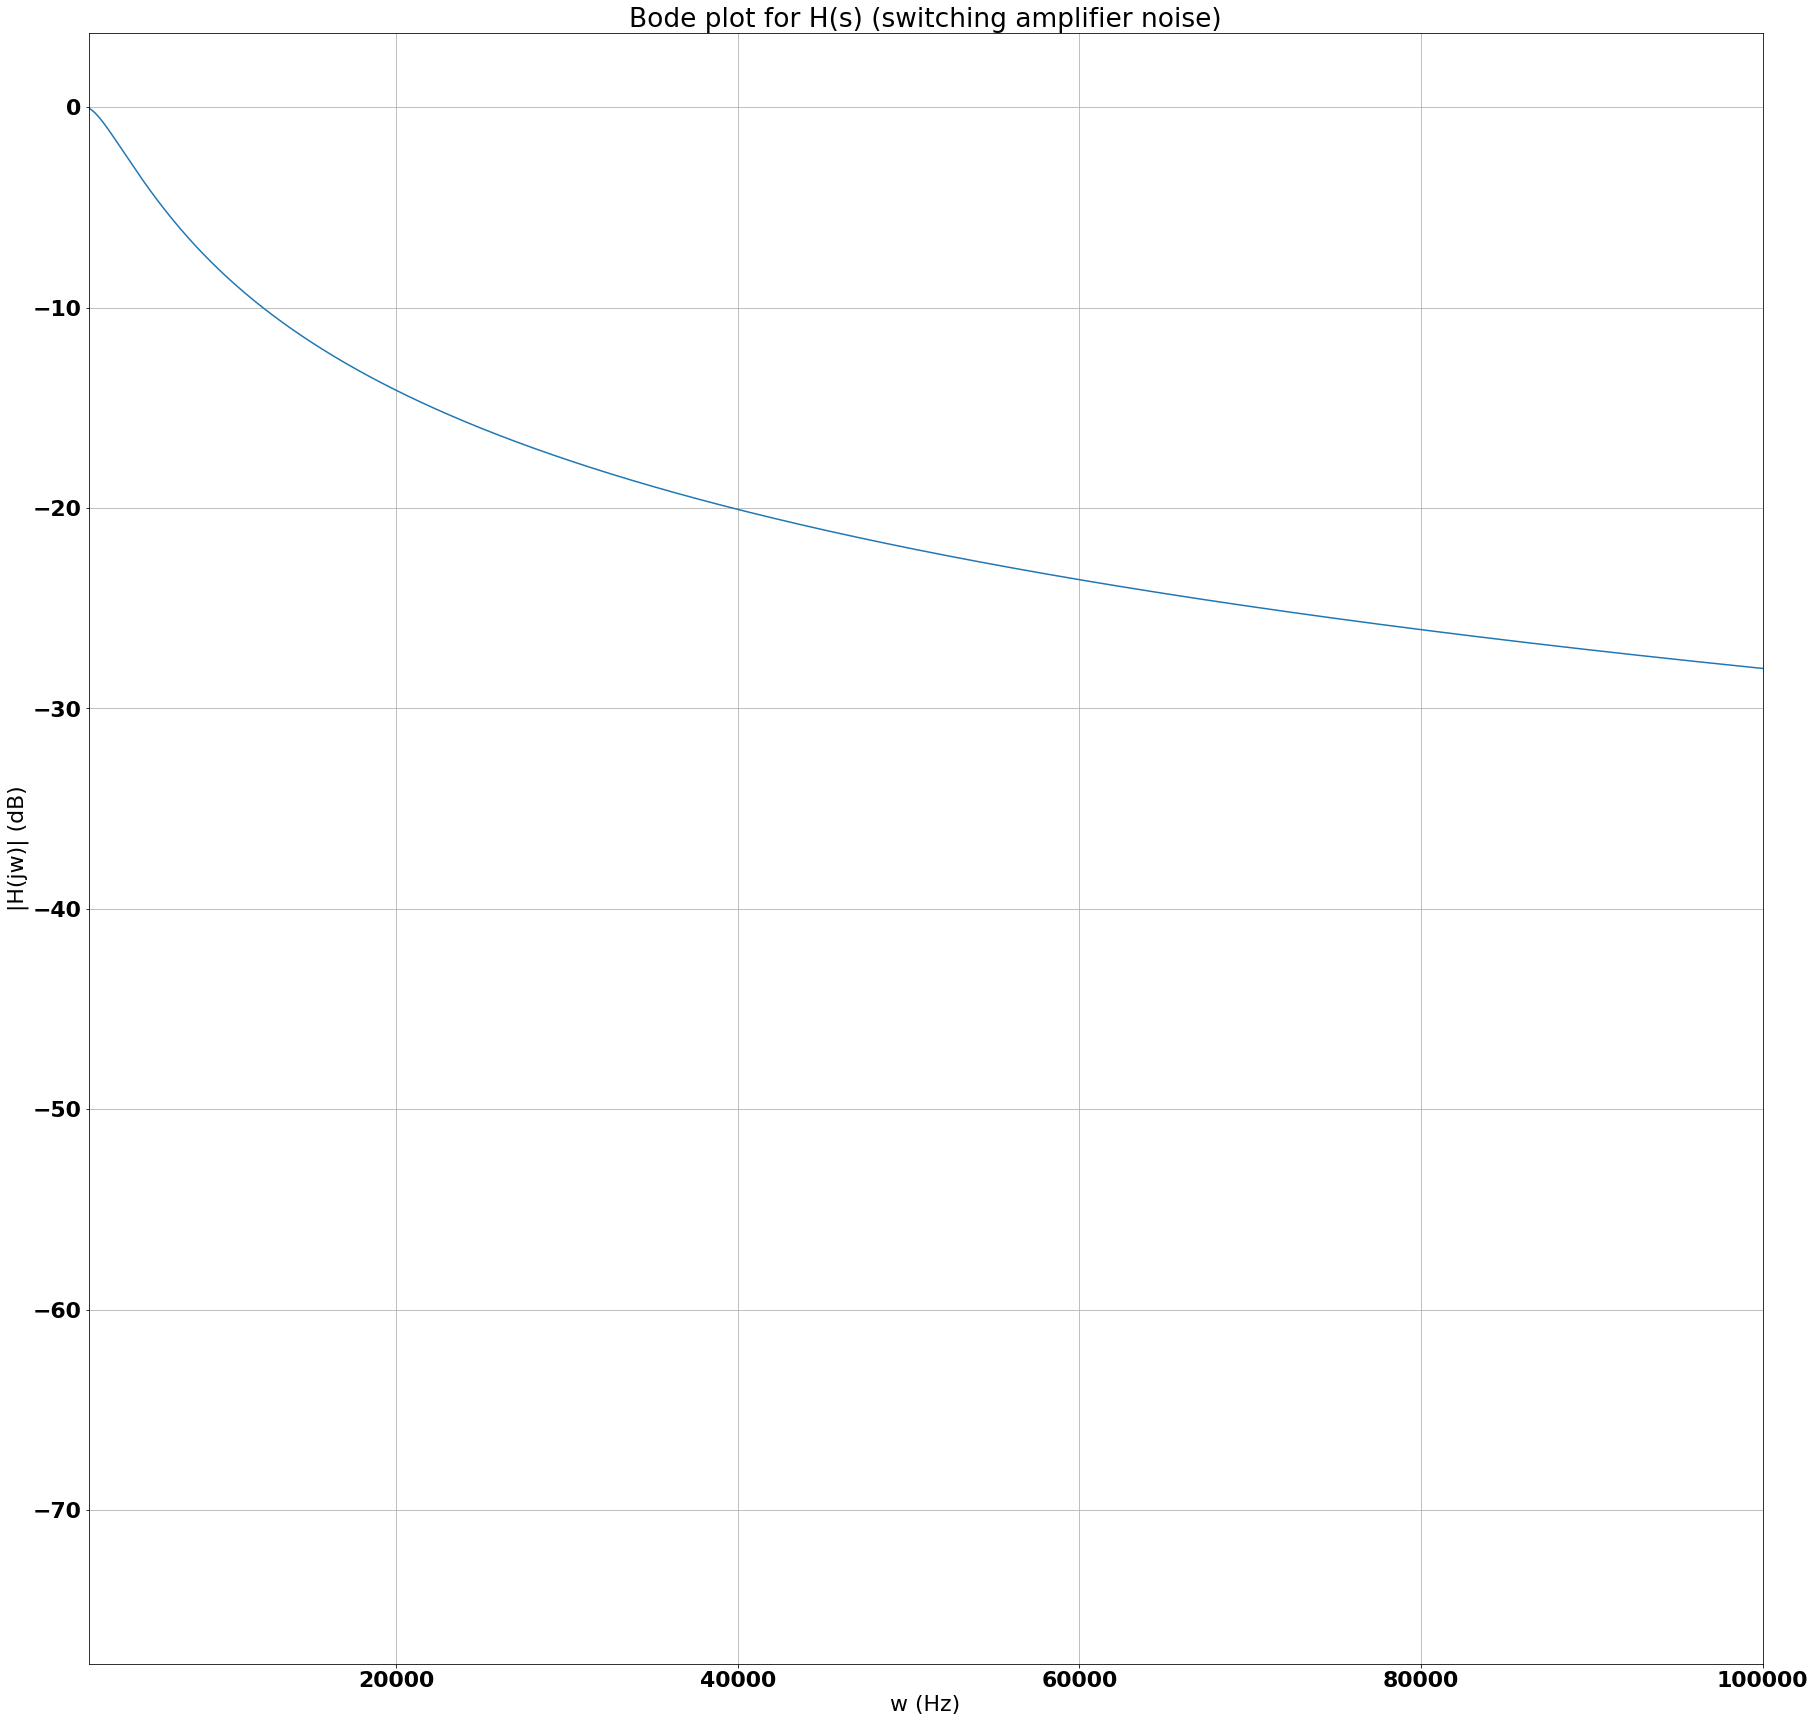
\includegraphics[scale = 0.2]{Figure 2022-04-20 163927 (9).png}
    
    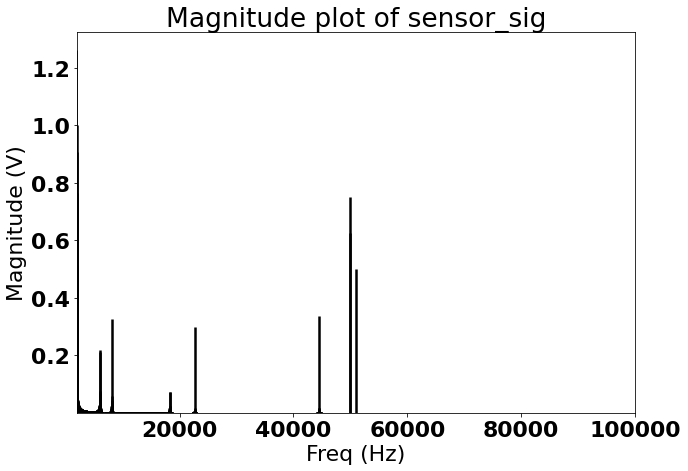
\includegraphics[scale = 0.5]{Figure 2022-04-20 163927 (4).png}

    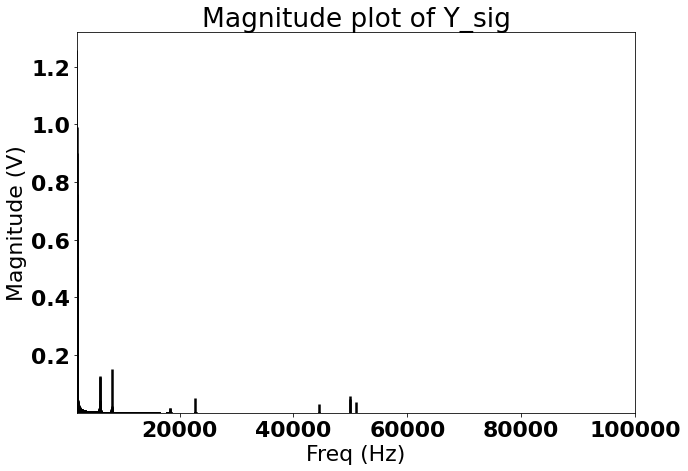
\includegraphics[scale = 0.5]{Figure 2022-04-20 163927 (15).png}
    
    \paragraph{} The bode plot shows how by 43,000 Hz, attenuation has reached -21dB. Considering the huge spike in noise at 50,000 Hz, reaching the expected attenuation before then is vital. 
    
    \paragraph{} For the fourth problem area, we're concerned with frequencies greater than 100kHz being completely attenuated. So, we're concerned with magnitudes reaching less than 0.05V after 100kHz.
    
    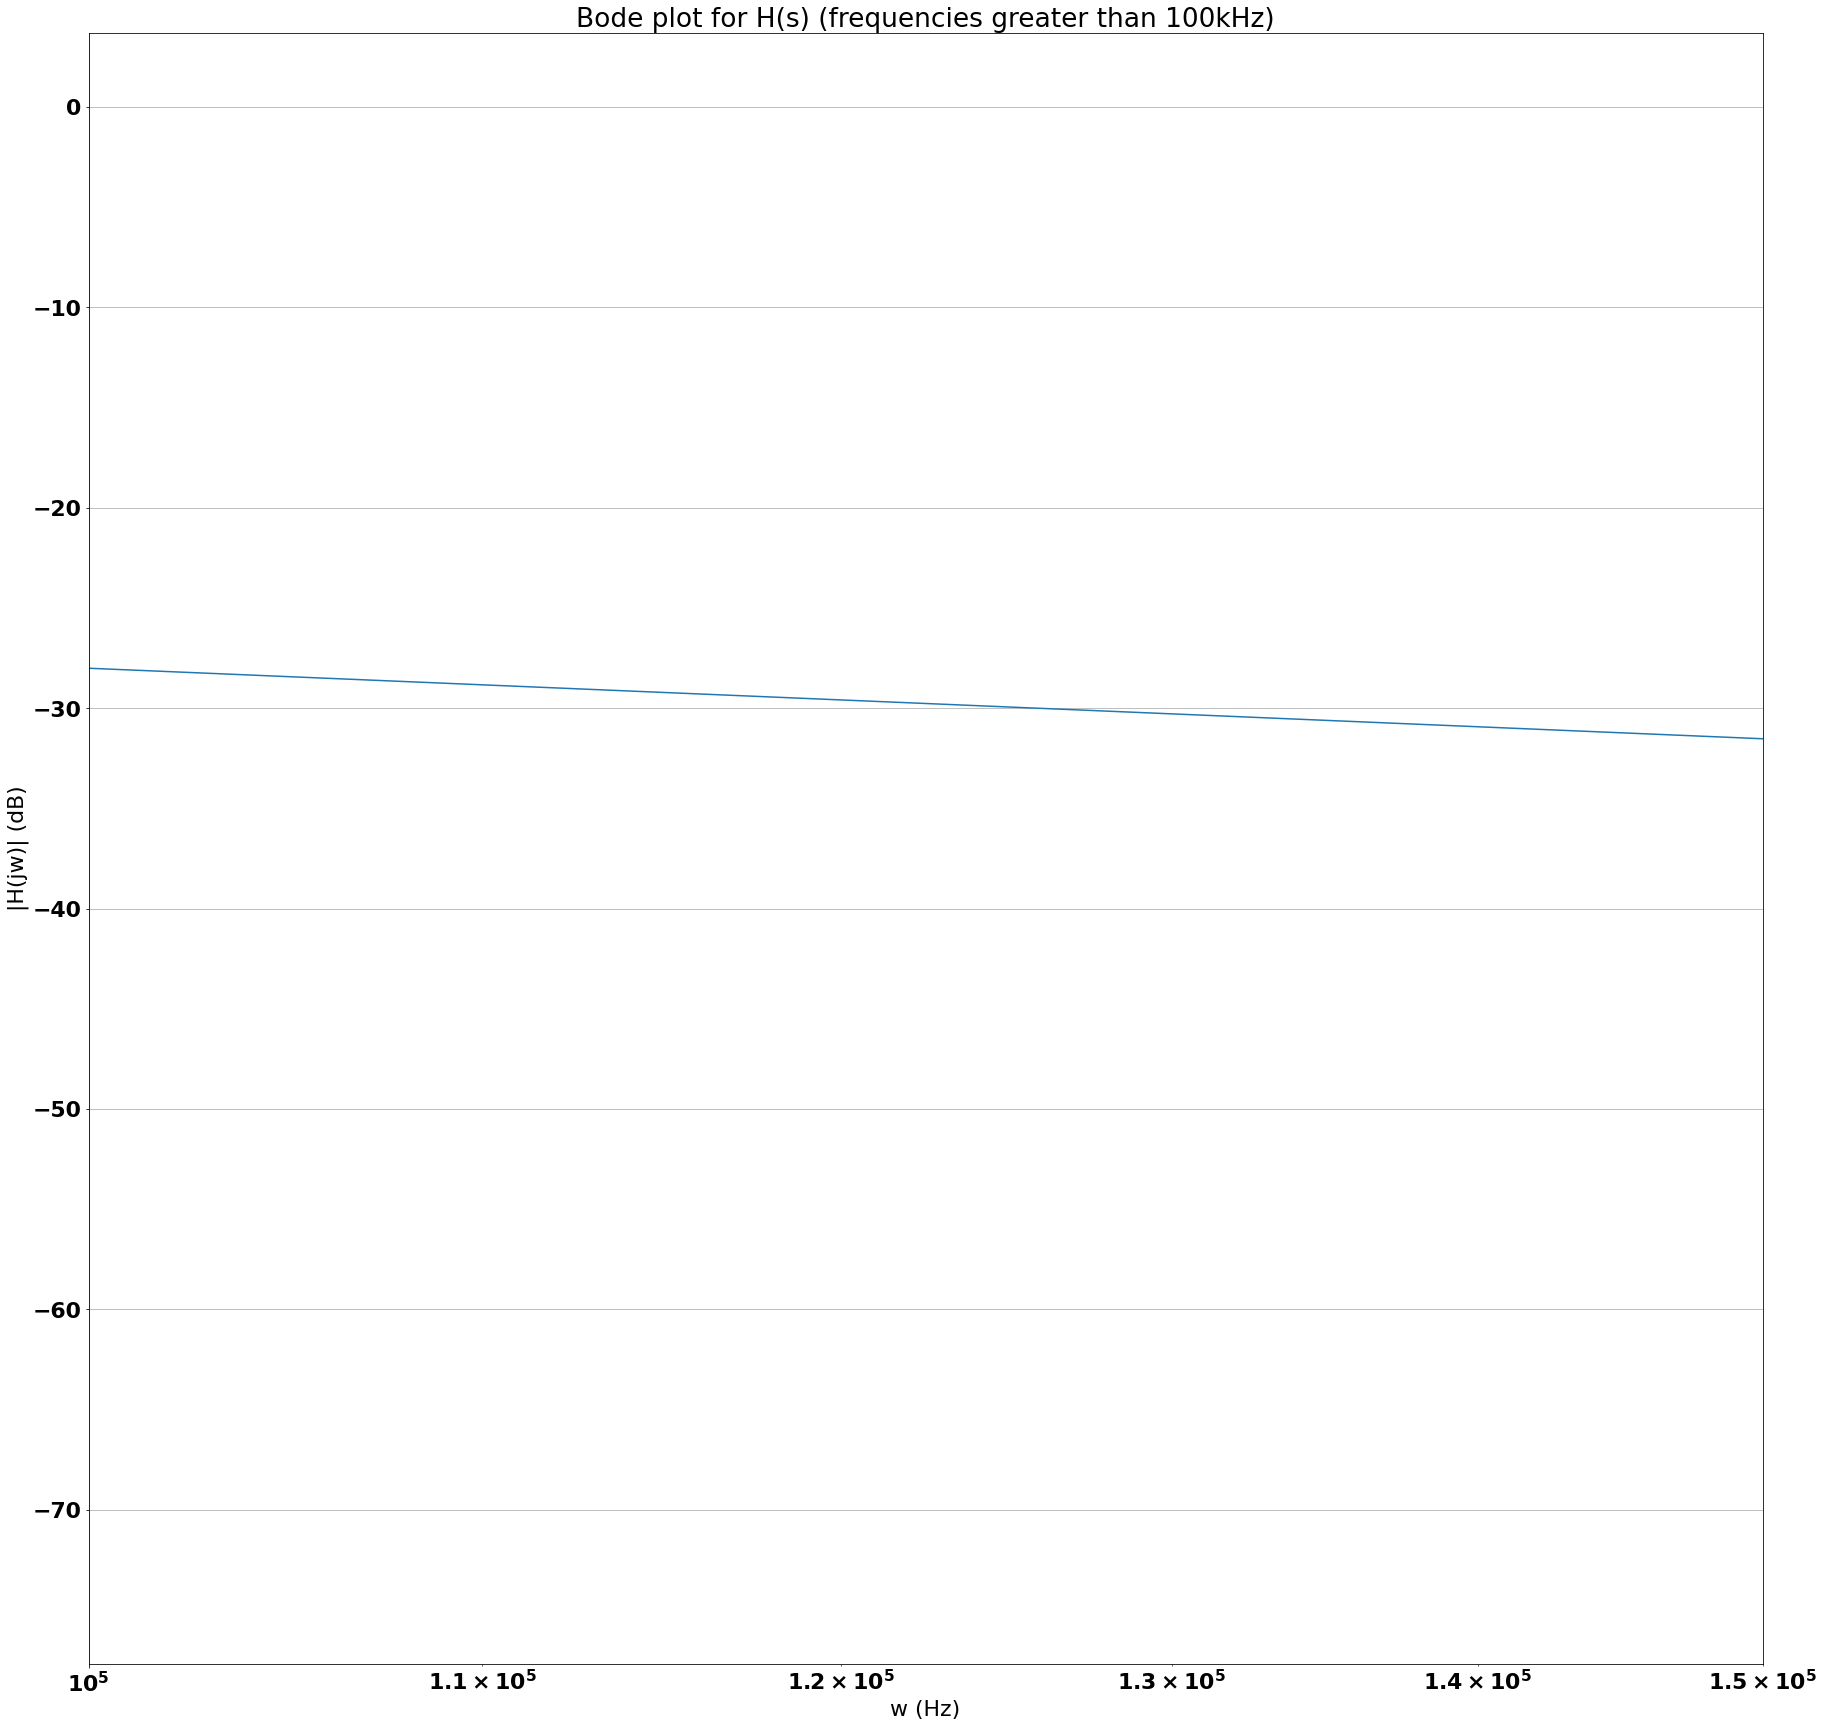
\includegraphics[scale = 0.2]{Figure 2022-04-20 163927 (10).png}
    
    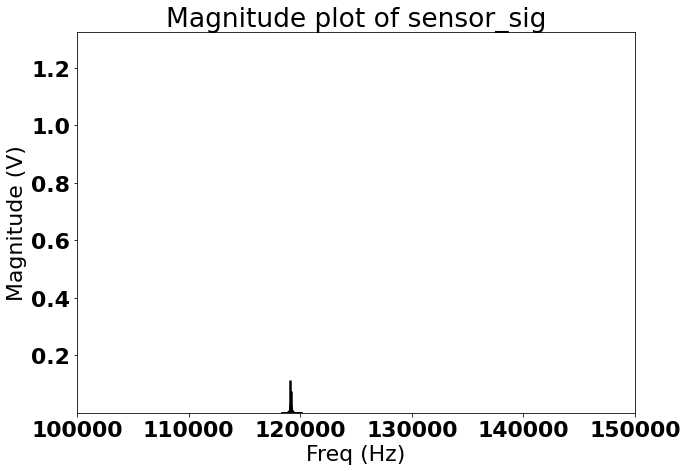
\includegraphics[scale = 0.5]{Figure 2022-04-20 163927 (5).png}

    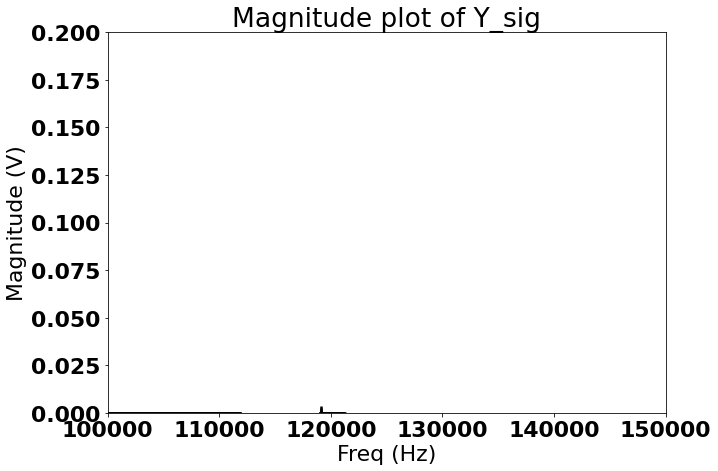
\includegraphics[scale = 0.5]{Figure 2022-04-20 163927 (16).png}
    
    \paragraph{} The input signal and output signal to the filter are displayed on two different y-scales. Considering how small the output signal's magnitude is, the frequencies greater than 100kHz are being completely attenuated.
    

\section{Error Analysis}

%This section will discuss error analysis of the experiment. Since this lab %deals with ideal simulation there shouldn't be any sources of error, so %instead this section can be used to describe any difficulties you had during %lab and how you solved them. Alternatively, if you couldn't get the %experiment to work, which is okay, you need to use this section to explain why %you couldn't get it to work to earn full points. 

\paragraph{} The main difficulty I encountered was filtering out all of the jargon from the problem description and trying to understand what I needed to do. The execution was the easy part, since I had access to old lab reports with relevant information. 

\section{Questions} %also address any deliverables not yet put in yet
    \begin{enumerate}
        \item Earlier this semester, you were asked what you personally wanted to get out of taking this
course. Do you feel like that personal goal was met? Why or why not?
        \paragraph{} My goal was certainly met. I learned a great deal more about programming in Python and its plotting capabilities. 
    \end{enumerate}

\section{Conclusion}

%Discuss briefly what you learned in this lab and whether or not you feel the %lab was successful. Include any recommendations for future labs as this is a %learning experience for all of us. Discuss any insights you gained from this %lab and how that will affect future work. \textit{Note: The bibliograhpy %needs to be on its own page.}

    \paragraph{} During lab 12, I learned how to apply what I've learned about filters and bode plots in a practical application. The lab was certainly a success and encouraged out-sourcing for information. I thought the imposition of restricting us to not collaborate with our fellow classmates didn't simulate a work environment well, but made sure we individually knew the information and how to apply it.    
    
    Github: \url{https://github.com/SethCram} 

\end{document}